\section{Strategia di swing-up}
Per lo swing-up uso il metodo di Ljapunov.
%così come descritto in [Astrom Furuta swinging up a pendulum by energy control].
%todo ref
Ricavo l'energia del solo pendolo e la uso per cercare una funzione
di controllo di Ljapunov.

\subsection{Energia del pendolo}
\label{subsec:energia-pendolo}
L'energia del solo pendolo è data da
\begin{align*}
    E &= T + V\\
      &= \frac 1 2 I \dot \theta^2 + mgl(\cos\theta-1)
    \numberthis \label{eq:energia-pendolo}
\end{align*}
dove ho scelto il potenziale in modo che si annulli quando $\theta=0$. Voglio studiare che effetto ha un accelerazione del perno sul pendolo. Risolvo l'equazione di eulero:
\begin{equation*}
    \totald t \partiald {\dot \theta} {\mathcal L} - \partiald {\theta} {\mathcal L} = -lma \cos \theta
\end{equation*}
dove $\mathcal L$ è la Lagrangiana del solo pendolo e a secondo membro compare il momento torcente che l'accelerazione $a$ imprime al pendolo.
Ottengo
\begin{equation}
    I \ddot \theta - mgl\sin \theta + mal \cos \theta = 0
    \label{eq:moto-pendolo}
\end{equation}
%todo qui bisogna sistemare un po' i simboli
e posso usare le due equazioni \eqref{eq:moto-pendolo} e \eqref{eq:energia-pendolo} per calcolare la variazione di energia istantanea che produce l'accelerazione $a$ lungo la traiettoria del moto.
Ottengo
\begin{equation*}
    \begin{aligned}
        \frac{dE}{dt}
        &= \totald t \left(\frac 1 2 I \dot \theta ^2 + mgl \cos \theta  \right) \\
        &= I \dot \theta \ddot \theta - mgl \sin \theta \cdot \dot \theta \\
        &= -mal \cos \theta \cdot \dot \theta
        .
        \label{eq:effetto-energia}
    \end{aligned}
\end{equation*}


\subsection{Funzione di controllo di Ljapunov}
Cerco una funzione di controllo di Ljapunov.
Prendo
\begin{equation}
    V = V(\b x) = \frac 1 2 E^2
        \label{eq:lyapunov-energy}
\end{equation}
e cerco una strategia di controllo $a$ per cui
\begin{equation*}
    \frac{dV}{dt}(\b x) < 0 \text{ con } \b x \neq \b 0,
\end{equation*}
secondo la proposizione~\ref{prop:condizione-sufficiente-ljapunov}.
Calcolo la derivata
\begin{align*}
    \frac{dV}{dt} &= \totald t \left( \frac 1 2 \dot E^2\right) \\
    &=  E \dot E \\
    &=  E (-mal \dot \theta \cos \theta) \numberthis\label{eq:dvdt}.
\end{align*}
La scelta più semplice è definire $a$ come funzione a tratti:
\begin{equation}
    a = \left\{
    \begin{aligned}
         &a_{\max}\sign{\dot \theta \cos \theta} &\text{ se } E < 0 \\
         -&a_{\max}\sign{\dot \theta \cos \theta} &\text{ se } E > 0 \\
         &0 &\text{ altrimenti}
    \end{aligned}
    \right.
    \label{eq:bang-bang}
\end{equation}
con $a_{\max}$ l'accelerazione massima possibile per il sistema.
La figura~\ref{fig:energy-control} mostra che questa strategia porta il sistema a
zero.

\begin{figure}
    \centering
    \begin{subfigure}[b]{0.48\textwidth}
        \centering
        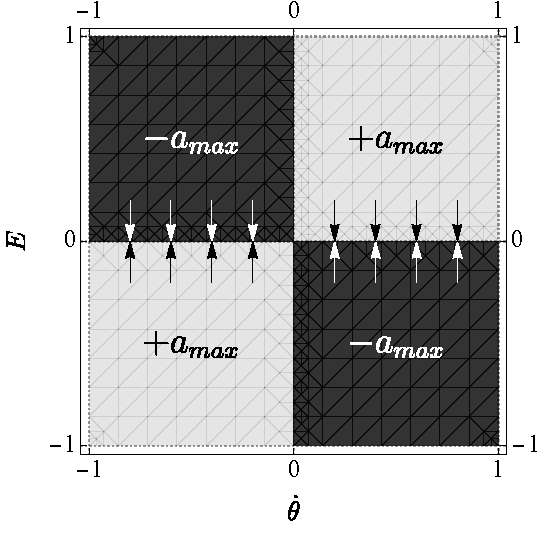
\includegraphics[width=\textwidth]{assets/energy-control1}
        \caption{$\cos\theta < 0$}
    \end{subfigure}
    \hfill
    \begin{subfigure}[b]{0.48\textwidth}
        \centering
        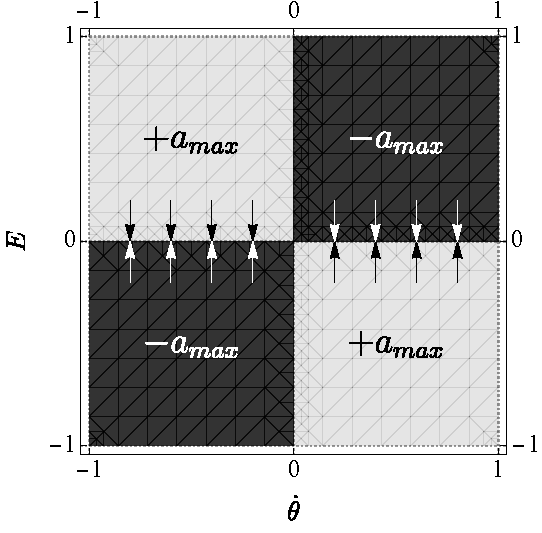
\includegraphics[width=\textwidth]{assets/energy-control2}
        \caption{$\cos\theta > 0$}
    \end{subfigure}
    \caption[Swing-up con funzione segno]{Strategia di swing-up con funzione segno.
    Nel grafico, il colore indica l'intensità dell'accelerazione $a$: il bianco
    corrisponde a un accelerazione verso destra e il nero ad un accelerazione verso sinistra.
    In modulo, l'accelerazione è sempre uguale. L'effetto del controllo, rappresentato dalle frecce, è
    di portare il sistema nella configurazione in cui $E = 0$.} %todo
    \label{fig:energy-control}
\end{figure}

\begin{figure}
    \centering
    \begin{subfigure}[b]{0.48\textwidth}
        \centering
        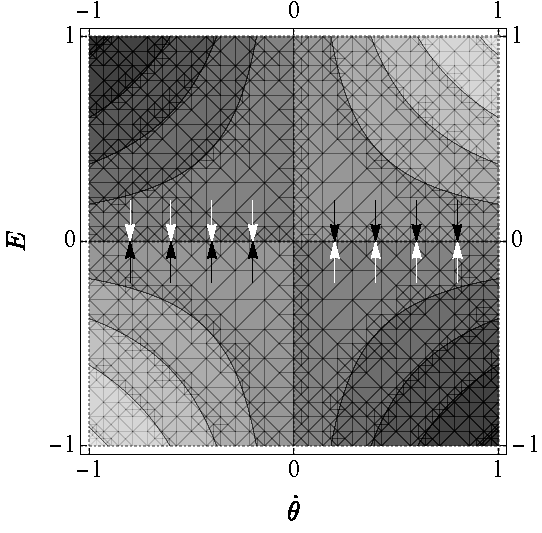
\includegraphics[width=\textwidth]{assets/energy-control3}
        \caption{$\cos\theta < 0$}
    \end{subfigure}
    \hfill
    \begin{subfigure}[b]{0.48\textwidth}
        \centering
        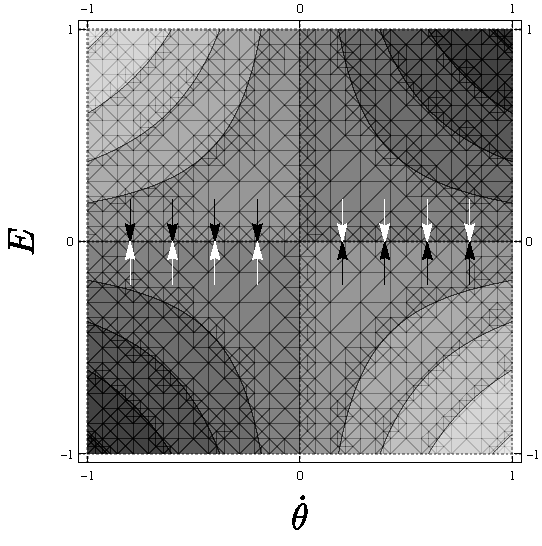
\includegraphics[width=\textwidth]{assets/energy-control4}
        \caption{$\cos\theta > 0$}
    \end{subfigure}
    \caption[Swing-up con tangente iperbolica]{Strategia di di swing-up con
    tangente iperbolica.
    Nel grafico, il colore indica l'intensità dell'accelerazione $a$: più è tendente al bianco, più è forte l'accelerazione verso destra e viceversa per il nero.
    L'effetto del controllo, rappresentato dalle frecce, è
    di portare il sistema nella configurazione in cui $E = 0$. I colori
    mostrano come questa strategia di controllo sia meno brusca della \eqref{eq:bang-bang}.} %todo
    \label{fig:energy-control-better}
\end{figure}

La funzione segno nella~\eqref{eq:bang-bang} la rende difficile da studiare
ed estremamente sensibile al rumore (la minima oscillazione costringe il motore
a passare istantaneamente da potenza zero a potenza massima).
Considero l'alternativa
\begin{equation}
    a = a_{\max} \tanh(E \dot \theta \cos \theta).
    \label{eq:control-strategy-tanh}
\end{equation}
Dimostro che la~\eqref{eq:lyapunov-energy} con $a$ definito come
nella~\eqref{eq:control-strategy-tanh} è una funzione di controllo di Ljapunov.
Uso la~\eqref{eq:dvdt}:
\begin{align*}
    \frac{dV}{dt} &=  E (-mal \dot \theta \cos \theta)\\
    &= -Eml \dot \theta \cos \theta \cdot a_{\max} \tanh(E \dot \theta \cos \theta). \numberthis\label{eq:a-ljapunov}
\end{align*}
ed è immediato verificare che la~\eqref{eq:a-ljapunov} è sempre negativa.
La~\eqref{eq:control-strategy-tanh} è rappresentata in figura~\ref{fig:energy-control-better}.

Concludo osservando che la strategia che ho mostrato in questo paragrafo
non tiene conto della posizione del carrello sulla rotaia.
È quindi necessario passare alla strategia di stabilizzazione
una volta che il pendolo ha raggiunto la verticale.